\chapter{The French nuclear bet} \label{chap:nuclear_bet}

%%%%%%%%%%%%%%%%%%%%%%%

\section{Introduction} \label{sec:introduction_chap2}
The first oil shock provoked the engagement of France in an unprecedented nuclear program, which would make it up to now the country with the highest share of nuclear in its power mix.
The first Contract Program was launched in 1969. A batch of six reactors of 900 MWe was ordered (the CP0 batch) and their construction started in 1971. But the 1973 oil embargo triggered a more ambitious nuclear program. In early 1974, 18 identical reactors of 900 MWe were ordered (CP1 batch). They were followed in late 1975 by 18 new reactors: 10 reactors of 900 MWe (CP2 batch) and 8 of 1300 MWe (CP4 batch). 12 additional reactors of 1300 MWe were ordered in 1980 (P'4 batch). Finally, in 1984, 4 reactors of 1450 to 1500 MWe (N4 batch) concluded this nuclear policy \citep{Boccard2014}.
These massive orders have shaped power production in France ever since. In 2015, these nuclear plants produced 78\% of the country's electricity. Along with a 12\% of hydropower production, it leaves only around 10\% for all other sources of power \citep{RTE2014}.

But these power plants are now reaching the end of their lifetime. The reactors were initially designed to last for 32 years at nominal power and 40 years at 80\% of their nominal power \citep[p. 31]{Charpin2000}. In practice, the 40-year threshold is used by the national authority on nuclear safety, the ASN. These reactors are now reaching this 40-year limit. The first ones will be the two reactors in Fessenheim, which will turn 40 years old in 2017.

The lifetime of these nuclear plants can be extended if retrofit works are undertaken. 
A new report by the French 'Cour des Comptes'\footnote{
	The Court of Auditors (in French Cour des Comptes) is a quasi-judicial body of the French government charged with conducting financial and legislative audits of most public institutions} 
estimated at \euro 100 billion the cost of retrofitting the plants up to 2030 \citep{CourdesComptes2016}. Should all plants be retrofitted? And more generally, what is the future of nuclear energy in France?
These questions are now at the heart of public debate. The diversity of opinions on this matter was highlighted by the French National Debate on Energy Transition in 2012. The views on the future of nuclear generation in France ranged from a fully maintained nuclear share, to partial retrofit strategies, to a full and early phase-out \citep{DNTE_gt2}. 

France is now at a crossroad. The economics of this decision crucially depend on the cost of nuclear, both new and retrofitted; but these are subject to significant uncertainty. A combination of recent setbacks in the nuclear industry has raised some doubt about the future cost and safety of this technology.
For new nuclear reactors, the most famous example is the significant cost overrun of the EPR at Flamanville (France). The project was initially estimated at \euro 3 billion, but this estimate has increased progressively up to \euro 10.5 billion in 2015 \citep{Garric2015}, and there are still concerns about the safety of its vessel \citep{Hir2015}. For retrofitted nuclear, the estimation may also be optimistic, as unexpected delays often occur in such megaprojects. For example, in the plant of Paluel, the replacement of steam generators has led to the fall of one steam generator of 465 tonnes, which requires safety inspection and will cause delays \citep{ASN2016}. Safety concerns about current vessels have also led to stopping nuclear reactors in winter, threatening security of supply \citep{Monicault2016}.

Other uncertainties must also be accounted for, in particular those concerning the level of demand and \coo\ price. The level of demand can be affected by economic growth or downturn, by energy efficiency and the development of new uses like electric cars. \coo\ price can impact the relative competitiveness of gas and coal, but also renewables backed up by gas. This \coo\ price depends on political will, which is difficult to anticipate.

Given these uncertainties, what are the policy options available, and what are their risks and benefits? 
The current debates suggest that there is no silver bullet, no single optimum strategy for all plausible values. Thus, we aim to find a robust strategy, i.e. a strategy that "performs relatively well --compared to alternatives-- across a wide range of plausible futures" \citep{Lempert2006}. 
%Our aim is also to identify trade-offs between possible strategies and the vulnerabilities of each strategy -- that is, combinations of model parameters in which the strategy performs relatively poorly. 
To do so, we combine the cost-minimizing optimization model of the French power sector FLORE with the framework of Robust Decision Making \citep{Lempert2006}, in a way similar to \citet{Nahmmacher2016}. This RDM framework combines scenario-based planning with statistical analysis, in order to identify robust strategies, vulnerabilities and trade-offs. We apply it to the results of nearly 3,000 runs made with the FLORE model. 
Our paper aims to provide insight for the current debate in France concerning the retrofit of existing nuclear plants. More generally, it also explores the importance of uncertainties related to nuclear energy in power system planning, and could thus contribute to the debates in other European countries, in particular Germany and Switzerland.

In section \ref{sec:plausibleValues}, we examine in detail the ranges of uncertainty. These ranges will be used for the parameters of our model FLORE, which is introduced in \cref{sec:modelDescription}. We present the RDM framework in \cref{sec:method} and apply it in \cref{sec:results} to identify robust strategies. Finally, we compare our results to the French official scenarios in \cref{sec:comparison}. \Cref{sec:conclusion2} outlines the conclusions.


%%%%%%%%%%%%%%%%%%%%%%%%%%%
%%%%%%%%%%%%%%%%%%%%%%%%%%%%%%%%


\section{The uncertainty ranges in the literature}
\label{sec:plausibleValues}

\subsection{Overview}
Various elements stretch the range of plausible future costs for both retrofitted and new nuclear.

On one hand, the recent literature and events about nuclear costs presents arguments supporting the idea of increasing costs in the future:
\begin{description}
	
	\item [Negative learning-by-doing] The French nuclear industry has been facing "negative learning-by-doing" in the past, although it benefited from a very favourable institutional environment \citep{Grubler2010}.
	
	\item [Increased regulatory pressure on safety] Increased regulatory pressure can increase costs \citep{Cooper2011}. In particular, the Fukushima accident has led the French nuclear regulator, the ASN, to impose new safety measures.
	
	\item [Recent and unexpected cost surge]: the EPR technology in Flamanville (France) has been delayed several times, and its cost tripled.
	The EPR in Olkiluoto (Finland) is also facing several difficulties.
	This is raising doubts about the ability of EDF to build power plants of the EPR technology.
	As to retrofitting the historic power plants, the first retrofit has led to an incident which may cause delays and significant cost increases\footnote{
		on March 31, 2016, a steam generator of 465 tonnes and 22m high fell during its replacement operation};
	
	\item [High contract price for nuclear] In the UK, EDF signed a contract at 92.5~\pounds/MWh (127~\euro/MWh at 2015 exchange rate of Eurostat\footnote{\url{http://ec.europa.eu/eurostat/web/exchange-rates/data/main-tables}}) and indexed on inflation, which means the nominal price will be higher when the plant starts to produce. The exact costs of the French EPR are difficult to assess as they are not publicly displayed. This market price is thus an important clue as to the cost of this technology.
	
	\item [Unexpected stops] The discovery of anomalies has led to reinforced controls. As a consequence, in October 2016, 12 reactors out of 58 were stopped to check the resistance of their steam generators \citep{Monicault2016}. This lead to concerns about the security of supply and the future load factor of these plants, which is a key parameter of their value \citep{IEA2015}.
	
	\item [Risks and insurance costs] The Fukushima accident prompted a renewed interest on the question of insurance costs from the French court of audit \citep{CourdesComptes2012}. This insurance should match the criticality of nuclear, i.e. the probability of an accident multiplied by severity of the consequences. Up to now, the French nuclear operator EDF has benefited from a limited liability. But both probability and damage costs are difficult to estimate. To give an idea of these uncertainties, \citet{Boccard2014} estimates this insurance cost at 9.6 \emwh, while \citet{Leveque2015} provides an expected cost below 1 \emwh. 
	
	\item [Decommissioning and waste management] No decommissioning has been finished yet, so the total cost is difficult to estimate. The first nuclear installation to be decommissioned in France, Brennilis, saw its cost multiplied by twenty compared to initial estimates. And in a novel report, a commission of the French Parliament reckons that the cost of dismantling might be underestimated in France \citep{AN2017}.
	As to waste management, a project called Cigeo is planned to store highly radioactive long-lived wastes. Its cost was estimated at between 15,9 and 55 billion euros in 2002 by the national radioactive waste management agency, ANDRA \citep[p. 142]{CourdesComptes2012}.
	
\end{description}

On the other hand, constructing several reactors of the same type can lead to learning-by-doing in the construction process. Standardization reduces lead times and thus reduces the cost of this technology. The size of reactors is also positively correlated with cost \citep{Rangel2015}, so a standardized approach with smaller reactors could thus stop the negative learning-by-doings and even decrease the future costs of nuclear.

These elements should encourage carefulness when assessing the future costs of nuclear. They entail that a wide range of costs can be considered as \textit{plausible}, in the sense that they cannot be immediately dismissed since some elements support them. In the next sections, we examine what could be the future cost of retrofitted and new nuclear, based on the current literature.


\subsection{Cost of retrofitted nuclear plants}

\subsubsection{Historical costs}

The cost of the French nuclear reactors has been the focus of a few papers.
The first official report on the historic French nuclear program was made by \citet{Charpin2000}.
It was later analyzed by \citet{Grubler2010}, who evidenced cost escalation in time, which he coined as "negative learning-by-doing".
After the Fukushima accident, the French court of audits undertook a comprehensive analysis of the costs and safety of French nuclear reactors. Based on this report, \citet{Boccard2014} revealed larger than expected operation costs for French reactors: 188 \euro/kW/year, or 28.5 \emwh\ with the historical load factor. This value is a key determinant of the cost of retrofitted nuclear, since fixed capital costs are already amortized to a large extent. And this estimate is much higher than the value suggested by \citet{IEA2015} at 13,3 \emwh.
Using the same report, \citet{Rangel2015} also noticed a cost escalation, but revealed a learning curve within technologies of the same type and size.


\subsubsection{Costs of retrofitting}
These old reactors now reach the end of their planned lifetime, initially intended to be 40 years\footnote{
	French reactors were initially designed for a lifetime of forty years, with a count start at their first nuclear reaction. In the US, lifetime is counted from the first layer of concrete.
}.
These lifetimes can be extended, but only if some upgrade work is performed. A new report published by the French court of audit \citep{CourdesComptes2016} provides the costs estimated by EDF\footnote{Electricité de France, the main operator of the nuclear fleet in France.} to retrofit its nuclear fleet and bring safety up to post-Fukushima standards. According to EDF, an investment of \euro 100B is required by 2030: 74.73 in CAPEX and 25.16 in OPEX \citep{CourdesComptes2016}.
Between 2014 and 2030, 53.2 GW will reach 40 years, yielding an average additional cost of 1,404 \euro/kW.

In addition to these overnight capacity costs, the cost per unit of energy produced is influenced by capital cost, load factor and lifetime.

Financial costs are highly dependent on the rate at which capital is borrowed. 
In France, \citet{Quinet2013} recommends to use a rate of 4.5\% for public investments.
The IEA uses a rate of 5\%, which we use for our best-case scenario, to account for financial costs.
We use a rate of 10\% for our worst-case scenario, following \citet{Boccard2014}.

For the load factor, we use a best case based on the estimates by \citet[p. 116]{CourdesComptes2016}, which shows that the availability of French nuclear plants has been up to 83.5\% since 2005. In 2012, the load factor was down to 73\% in 2012, but considering the recent difficulties faced by French reactors, we use a load factor of 70\% as a worst case.

As to lifetime, we suppose that the investment of \euro 100B will enable the plant to run for 20 more years. This is currently the implicit assumption of EDF \citep[p. 13]{AN2017}, but there is significant uncertainty around this hypothesis. In France, nuclear plants are given license by periods of ten years. 
The French Authority of Nuclear Safety (ASN) seems willing to provide licenses for a ten year extension; but there is no certainty that it will give a second approval, ten years later, to go beyond fifty years of operation. 
It may decide to close some plants, or ask for additional investment at that time. However, the magnitude of the investment indicates that EDF is confident it will be able to run for twenty more years without incurring in large additional costs. Thus, this is our best-case hypothesis. We consider a worst case in which lifetime extension will be granted for ten years only. 


\subsubsection{Cost of a nuclear accident}
\label{ssec:accident}

The Fukushima accident has prompted a renewed interest on the question of insurance costs. The insurance cost should match the criticality of nuclear, i.e. the probability of an accident multiplied by severity of the consequences. However, both the probability of an accident and damage costs are difficult to estimate.

Damage costs depend on several assumptions about indirect effects, as well as on monetizing nature and human lives \citep{Gadrey2016}. Thus, an irreducible uncertainty remains here. To give an idea of these uncertainties, the Institute for Radiological Protection and Nuclear Safety (IRSN) estimated the cost of a "controlled" release of radioactive material between 70 and 600 billion euros \citep{CourdesComptes2012}. To give another reference, the Fukushima accident has been estimated at 160 billion euros by \citet{MunichRe2013}.

To assess the probability of a nuclear accident, two approaches coexist. The first one is the Probabilistic Risk Assessment (PRA). It consists in a technical bottom-up approach, which compounds the probabilities of failures which could lead to a core meltdown. This measure is used by regulators in the US \citep{Kadak2007}. Depending on regulators, this PRA varies from 10\textsuperscript{-4} to 10\textsuperscript{-6} per year and per reactor \citep{Ha-Duong2014}. In France, the probability of an accident which would release a significant amount of radioactivity in the atmosphere is estimated at 10\textsuperscript{-6} for current plants, and 10\textsuperscript{-8} for the EPR reactor \citep{CourdesComptes2012}. However, some uncertainty remains within the information that is not fully captured by this type of analysis, as suggested by the examples of Three Mile Island, Chernobyl and Fukushima. A wide discrepancy is observed at first glance between the expected number given by the PRA estimate and the number of observed nuclear accidents worldwide \citep{Ha-Duong2014}. 

This discrepancy has motivated another approach, based on the statistical analysis of past historical accidents. In particular, the Fukushima accident has prompted a renewal of research based on empirical estimates. \citet{Rangel2014} recall that most of the accidents occurred at the early stage of nuclear power plants. Continuous safety improvements might have improved security and brought it closer to PRA estimates. They also argue that the Fukushima accident has revealed the risks associated with extreme natural events and regulatory capture, thus opening the door for further improvements.

However, this second approach suffers from two short-comings. The first one is the low number of occurrences. Only two events are classified in the category of major accident, i.e. a level 7 on the INES scale - the INES scale, introduced by the International Nuclear Energy Agency, ranges nuclear events from 1 (anomaly) to 7 (major accident). Such a small sample hinders robust statistical analysis. Most studies thus estimate the probability of a larger pool of events by including events lower on the INES scale, but the gain in estimation accuracy comes at the cost of a change in the meaning of the results \citep{Rangel2014}. What is measured is not only the probability of major accidents occurring, but it also includes the probability of less dramatic events. 
The second shortcoming comes from the use of past, historical data. This does not enable to account for the potentially increased risks due to aging power plants, nor for the tense political situation with fears of terrorist attacks. 
This uncertainty can drastically change the cost of insurance. If we estimate the cost of insurance should match the criticality of nuclear, and if we assume the cost of a major nuclear accident to be 100 billion euros, as recommended by \citet{CourdesComptes2012}, then a probability of accident between 10\textsuperscript{-7} and 10\textsuperscript{-6} makes the insurance cost vary from 1.4~\emwh\ to 14.2~\emwh, as shown in \cref{tab:insurance}. 
And that range is in line with the requirement from the regulator for a core meltdown.

The point behind these figures is that the cost of insurance cannot be dismissed once and for all. Expectations of security improvements can explain an almost negligible value for nuclear insurance, while a more conservative view can lead to significantly higher estimates, up to 14 \emwh. 

\begin{table}
	\centering
	\caption{Estimated nuclear insurance costs for a damage cost of 100 billion euros.}
	\label{tab:insurance}
	\begin{tabular}{p{2cm}p{6cm}}
		\toprule
		Estimated probability of an accident \newline (per MW per annum) & Insurance cost (euro/MWh) \\
		\midrule
		$10^{-8}$  & 0,14 \\
		$10^{-7}$  & 1,43 \\
		$10^{-6}$  & 14,27 \\
		$10^{-5}$  & 142,69 \\
		\bottomrule
	\end{tabular}  
\end{table}


\subsubsection{Decommissioning and waste management costs}

A novel report by the French Parliament provides several clues as to the uncertainty surrounding decommissioning costs. 
Brennilis, an experimental reactor built in 1962, marks the first decommissioning of a nuclear power station in France. Although not achieved yet, the cost of decommissioning is currently estimated to be 482 million euros, around twenty times its initial estimate \citep{AN2017}.
This evolution leads to be cautious with the current cost assessments of other nuclear installations.
Even the technical feasibility of decommissioning is not granted yet. This is illustrated by the decision of EDF to postpone to 2100 the decommissioning of several experimental nuclear installations in order to have the time to develop new technologies for a safe decommissioning \citep{AN2017}.
Finally, there is a large divergence between the estimates of European operators. The accounting provision is generally between 900 and 1.3 billion euros per reactor, EDF's provision is only 350 million euros per reactor \citep{AN2017}. The argument of standardization is used to justify this lower cost estimate.
But due to the significant difference with other European operators, we also consider a worst-case scenario in which a doubling of current costs and provisions cannot be excluded.

As to waste management, a facility called Cigeo is planned to be built to serve as a repository for highly radioactive long-lived wastes. The cost of this project was estimated at between 15,9 and 55 billion euros in 2002 by the national radioactive waste management agency, ANDRA \citep[p. 142]{CourdesComptes2012}.
Since these costs will be incurred in a distant future, valuing this nuclear liability depends on the choice of a discount rate. \citet{Taylor2008} estimates a risk-free rate should be used. 
In France, the discount rate is fixed by the application decree 2007-243 of 23 February 2007 relative to ensuring the financing of nuclear accounting charges\footnote{décret 2007-243 du 23 février 2007 relatif à la sécurisation du financement des charges nucléaires}. 
The nominal rate must be lower than a four-year moving average of government bonds of constant maturity at 30 years, plus a hundred base points \citep[p. 110]{CourdesComptes2014}. This rate is subject to market fluctuations, which impacts the amount of accounting provisions and thus the cost of nuclear.
However, an increase in the cost of Cigeo from 16.5 to 36 billion euros would only increment generation costs by 1\% \citep[p. 282]{CourdesComptes2012}. This small sensitivity is due to the effect of discounting long-term costs. Given the uncertainty on costs and discounted rate, we consider another doubling of cost as our worst-case scenario.

In conclusion, decommissioning and waste management costs add another layer of uncertainty to generation costs. However, their overall impact, without being negligible, is mitigated by the discounting effects.


\subsubsection{Summing up}
Overall, there are at least eight sources of uncertainty for retrofitted reactors: the overnight capital cost of retrofitting, the cost of borrowing, the future OPEX, the length of lifetime extension (10 or 20 years), the future availability of nuclear plants and the costs of waste, decommissioning and insurance.
Using the most recent data available, detailed in \cref{tab:historical_costs} and \cref{tab:costs_grand_carenage}, we compute that, in the best case, the cost of retrofitted nuclear would be 44 \emwh. But based on conservative assumptions detailed in \cref{tab:sensitivity_tests} in appendix, various sources of uncertainty could amount to an additional 51.5 \emwh. Plausible values for this technology thus range from 44 \emwh\ to 95.5 \emwh.


\begin{figure}[!ht]
	\centering
	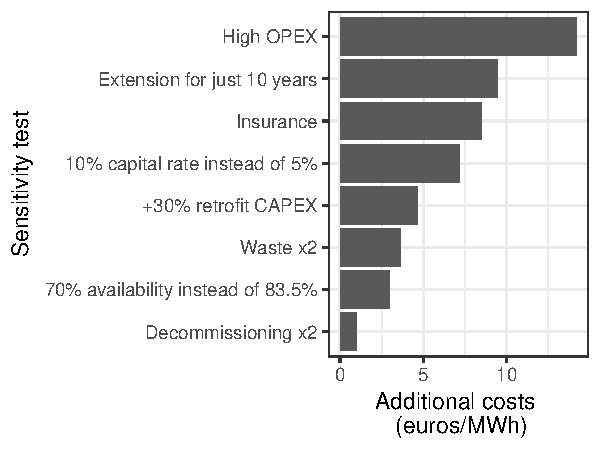
\includegraphics[height=5cm]{figures/sensitivity_tests.pdf}
	\caption{Plausible additional costs for retrofitted nuclear compared to a best case of 44 \emwh}
	\label{fig:sensitivity_tests}
\end{figure}

\subsection{Cost of new nuclear plants}

In parallel to retrofitting its existing reactors, EDF has developed a new technology: the European Pressurized Reactor (EPR).
However, this model has also faced serious setbacks.
The yet unfinished reactor developed in France saw its cost rising from \euro 3 billion to \euro 10.5 billion.
In Finland, the construction work for an EPR reactor started in 2005 with a connection initially scheduled in 2009, but has so far been delayed until 2018.
In the UK, the EPR has been negotiated at 92.5 \pounds/MWh -- approximately 127 \euro/MWh at the exchange rate of 2015 given by Eurostat.

As to the future of the EPR cost, a tentative cost is estimated by \citet{Boccard2014} between 76 and 117 \emwh, for a total cost of \euro 8.5 billion (before its upwards adjustment to \euro 10.5 billion) when including back-end and insurance costs (he estimates insurance costs at around 9.6 \emwh). 
The high end is in line with the contract price of the Hinkley point reactor. A wide spread is found in the literature, from 76 \euro/MWh to 120 \euro/MWh.
In addition, the cost of nuclear has been shown to depend on safety pressure. For example, \citet{Cooper2011} showed that the Three Mile Island accident had a significant impact on cost escalation.
Consequently, any new incident could increase these current estimates. This creates additional uncertainty on future nuclear costs.
These significant uncertainties about future costs led some to qualify the nuclear option as a "bet" \citep{Leveque2013}.

This wide range of nuclear cost is critical, as it encompasses the current levels of feed-in tariffs for wind in France and its LCOE\footnote{
	The Levelized Cost of Electricity, or LCOE, is an economic assessment of the average cost of one unit of energy produced by a power-generated asset. It is equal to total discounted costs divided by total discounted generation over the lifetime of the asset.}
expected in 2050. 
In France, in 2014, onshore tariff was set between 55 and 82 \euro/MWh for a lifetime of 20 years (82 \euro/MWh for the first ten years, and between 28 and 82 \euro/MWh afterwards, depending on wind conditions)\footnote{
	Note that the wind developer must pay for connection to and upgrade of the distribution network to access this FIT.
}.
Wind tariffs in neighboring Germany were set at 59 \euro/MWh in 2015: 89 \emwh\ during 5 years and 49.5 \emwh\ afterwards \citep{EEG2014}.

Finally, it is important to note that new nuclear is expected to be costlier than retrofitted plants. The general idea is that a brown field project (a retrofitted plant) requires less investment than a greenfield project. Thus, we will focus on the cases in which new nuclear is costlier than retrofitted nuclear.


\subsection{Demand, CO2 price and renewable cost}
\label{subsec:demand}

There is some uncertainty on the demand level. This was highlighted during the National Debate on Energy Transition in France, which led to four contrasted demand scenario: SOB, EFF, DIV and DEC, in order of increasing demand (see \cref{fig:DNTE_scenarios} in appendix). 
Our reference scenario is in line with the DIV scenario, as it is closest to current projections by the French transmission line operator, RTE. It is roughly a scenario of flat demand. The most extreme scenarios were SOB, for low demand, and DEC, for high demand. We use these as our low and high case respectively, to account for all plausible values of demand.

For \coo, we use the official price used in French public investments as defined in \cite{Quinet2009}. In the central scenario, this price goes up to \euro 100 in 2030 to \euro 200 in 2050. In the short term, these prices are significantly higher than the price of emission allowances on the EU ETS market (which has stayed below 10 \euro/\coo\ on the EEX market in the past year) and there is no reason to think that the EU ETS price might be higher, even with the proposition of back-loading some allowances in the future \citep{Lecuyer2016}. 
We also consider a variant with low \coo\ price, in which we divide the official price by a factor of 2. 
It thus attains 50 euros in 2030 and 100 euros in 2050. Such a high price reflects the implicit view in all scenarios to phase-out coal and gas in the long-term, in order to avoid an increase of \coo\ emissions. They could also represent the price floor for \coo\ currently discussed in France. 

All these uncertainties thus raise the question of the optimal mix. However, the LCOE metric does not account for "integration costs" \citep{Ueckerdt2013}. 
Nuclear has the advantage of being a dispatchable power source, while wind and solar PV are variable. As a consequence, their value decreases as their penetration rate increases, although the magnitude of this decrease is specific to the power system \citep{Hirth2016a} and to the renewable technology characteristics \citep{Hirth2016}. This phenomenon of value drop is sometimes called "self-cannibalization effect". Using an optimization model of the entire power system enables us to capture these integration costs. Indeed, since the model finds the power system that satisfies demand at the least cost to society, wind or solar would only be installed if they are competitive.


\subsection{Related literature on power transition and nuclear}

Many studies have analyzed a low-carbon transition in the power sector, at a national level \citep{Fraunhofer2015} or a European level \citep{Jagemann2013, EuropeanCommission2012}. 
Focusing more specifically on nuclear, \citet{Bauer2012} study the cost of early nuclear retirement at world level, and show that the additional cost of enforcing a nuclear phase-out is an order of magnitude lower that the total cost of a climate policy. But this result might not hold true for France as the share of nuclear is much higher than the world average.

\citet{Linares2013} analyze the break-even overnight cost of nuclear, using an optimization model of the Spanish power sector. They come up with a medium estimate of 2,609 \euro/kW, and conclude that the cost-competitiveness of this technology is questionable given the cost estimates of new projects.

In France, the French Energy Agency, ADEME, produced a study of renewable penetration in 2050 \citep{ADEME2015}. However, they do not study the path between today and 2050: the power mix was built ex nihilo (greenfield optimization) in 2050 as an optimization with 2050 projected costs.
\citet{Petitet2016} study wind penetration in France, but without modeling the potential of hydro optimization to smooth wind penetration, and consider only cases in which nuclear is cheaper than wind - a debatable assumption, as we will show.

The uncertainties of power system planning have recently been emphasized by \citet{Nahmmacher2016}, who studies unplanned shocks in power systems using the same methodology as in this paper. But their study does not deal with unexpected costs of nuclear plants.

Our paper contributes to the literature in several points. The first and main one is to use a methodology of robust decision making to deal explicitly with the high uncertainty on nuclear costs. The literature as a whole shows a wide uncertainty on nuclear costs. Rather than using specific -- and controversial -- values, we propose a methodology to include this uncertainty in the decision-making process. This is an improvement compared to the pure cost-minimization, thresholds-based or sensitivity analyses. In addition, we provide new estimates on the cost of nuclear retrofit based on a novel report by the French government and, include a retrofit option in our analysis, rather than focusing on new plants. We also provide a model to study nuclear and renewables with around 12\% hydro and optimized pumped storage, while the literature has focused mainly on thermal power systems, and seldom on power system with a high share of hydro \citep{Hirth2016a, Linares2013}. Finally, we provide trajectories of nuclear for France, which is often difficult to represent properly in models covering a larger region because of its large nuclear fleet.



The next section introduces the model we use for our analysis.


%%%%%%%%%%%%%%%%%%%%%%
%%%%%%%%%%%%%%%%%%%%%%%%%%%

\section{Model description} \label{sec:modelDescription}

The French power model FLORE (\textit{French Linear Optimization for Renewable Expansion}) is an optimization model of investment and dispatch. It is based on representative technologies, with a particular focus on nuclear and hydropower modelling to reflect the specificities of the French power mix. All technologies are endogenous for both investment and dispatch, except for hydro capacities. Existing nuclear plants may be retrofitted for 20 years when they reach 40 years old, or they are decommissioned. Hydro resources from dams and pumping stations are dispatched optimally. In addition, all capacities are jointly optimized over the horizon, in order to provide a consistent trajectory of investments. France is represented as a single node. Hourly demand, net exports and \coo\ prices are exogenous. 

All the equations of the model are available at \url{http://www2.centre-cired.fr/Rubrique-de-services/flore/description}. In addition, an interactive online version of the model can be found at \url{https://qperrier.github.io/#app}. This open access should ensure transparency and reproducibility, as advocated by \citet{Pfenninger2017}.

\subsection{Generation technologies}

Twelve generation technologies are modeled: two renewable energies (onshore wind and solar PV), three fossil-based thermal technologies (coal plants, combined cycle gas turbine, open cycle gas turbine), three nuclear technologies (historical nuclear, retrofitted nuclear and new nuclear) and three hydro systems (run-of-river, conventional dams for lakes and pumped storage).
Investment in each technology is a choice variable of the model, except for hydropower and historical nuclear, which are exogenous.
Generation of each technology is a choice variable, except for run-of-river production, which is exogenously based on historical data.

The capacity of run-of-river and conventional dams is supposed to be constant, while the pumped hydro capacity is supposed to grow by 3.2~GW by 2050, with a discharge time of 20 hours, as in \citet{ADEME2013}.
Hydro storage and dispatch is optimized by the model, under water reservoir constraints and pumping losses.
Dams receive an amount of water to use optimally at each period.
Pumped hydro can pump water (although there are losses in the process), store it into a reservoir and release the water through turbines later on.

A particularity of the model is to represent explicitly the cost of extending the lifetime of nuclear power plants.
Nuclear plants normally close after 40 years, but their lifetime can be extended to 60 years, if upgrade costs are paid for.
For historical nuclear, we model a phase-out of the capacity of each power plant reaching 40 years.
The same year it reaches 40 years, this capacity of a historical nuclear plant is endogenously either extended for 20 years, or phased-out. 
Thus, each year, total investment in retrofitted plants is limited to the capacity of historical nuclear reaching forty years.

Hourly Variable Renewable Energy (VRE) generation is limited by specific generation profiles based on historical data for the year 2014.
Dispatchable power plants produce whenever the price is above their variable costs, unless they are limited by their ramping constraints.
At the end its lifetime, each capacity is decommissioned.
Power generation required for heat generation was on average 2\% of consumption, and never above 5\% of consumption in France in 2014 \citep{RTE2014}, so we do not model it.
The remaining capacity can be optimized for power generation.

\subsection{Model resolution}

The model optimizes new capacities at a yearly step from 2014 to 2050. The dispatch of generation capacities is computed to meet demand for six representative weeks at an hourly step. Each typical week represents the average demand of two months of real data, through 168 hours. For example, demand of Monday for week 1 represents the average demand, on an hourly basis, of all the Mondays in January and February. This is similar to having 24*7=168 time slices in the TIMES model\footnote{http://iea-etsap.org/docs/TIMESDoc-Intro.pdf} or in the LIMES-EU model\footnote{https://www.pik-potsdam.de/members/paulnah/limes-eu-documentation-2014.pdf}.
Demand is exogenous and assumed to be perfectly price inelastic at all times. Net export flows are given exogenously, based on historical data. 
The various demand scenarios we study represent the initial demand profile (domestic consumption plus exports) and change it homothetically, thus without altering the shape of peak or base demands.

The model covers France as a single region.
Each typical week is associated with i) a water inflow for run-of-river and dams, ii) an availability factor for conventional generation technologies for each representative week, to account for maintenance and iii) a production profile for renewable technologies (onshore wind and PV) based on historical production.

\subsection{Objective function}

The objective of the model is to minimize total system costs over the period 2014-2050.
The cost of each technology is annualized, both for O\&M and capital costs. 
Capital annuities represent the payment of the loan. 
In addition, using annuities allows us to avoid a border effect in 2050: the annual costs are still well represented at the end of the time horizon.

We use a 0\% rate of pure time preference, in order to give the same weight to the different years and generation up to 2050. This assumption is also made in the EMMA model \citep{EMMA} used for example by \citet{Hirth2016}.
Costs include investment costs, fixed O\&M costs, variable costs and costs due to ramping constraints.
To account for financing cost (e.g. the cost of borrowing), investment costs are annualized with a 5\% interest rate, as in \citet{Jagemann2013}.
Variable costs are determined by fuel costs, CO\textsubscript{2} price, plant efficiency and total generation.

In \ref{sec:plausibleValues}, we studied the range of plausible values for nuclear, highlighting eight sources of uncertainty. Looking at these specific cost items was necessary to understand the range of plausible costs for retrofitted nuclear, but we will not detail each of these items in our model, as it would lead to too many possibilities (and possibly overlapping ones). Instead, we will keep the OPEX fixed and make the CAPEX vary to cover the uncertainty range. This simplified approach allows a decision maker to use its own assumptions about each cost item, and use the resulting cost in euro per MWh to interpret our results.

All assumptions regarding investment costs (\cref{tab:Investment _costs}), fixed O\&M costs (\cref{tab:OM_costs}), CO\textsubscript{2} price (\cref{tab:CO2_price}), fuel prices (\cref{tab:Fuel_prices}) and net efficiencies (\cref{tab:Efficiencies}) can be found in appendix \ref{app:calibration}.

\subsection{Scope and limitations}

The objective function does not include grid costs explicitly.
However, for wind, the feed-in tariff we use includes grid connection costs, through the 'quote-part' paid by the wind developer to the network operator ERDF.
For nuclear plants, they will be most likely built on sites with grids already built. (However, the size of the new reactors is significantly higher: 1.6 GW against 0.9 GW for many French reactors. Some upgrade words on the network might be necessary.)

Demand is exogenous.
In the long-term, it means there is no price-elasticity of demand.
However, we model four demand scenarios to account for demand variability.

We do not model endogenous learning curves. As we model only France, it is a reasonable assumption that worldwide learning curve will not be significantly impacted. However, installing renewable could lead to learning at the industrial level for the installation phase.

We do not include capacity credits, as is sometimes found in the literature. Demand is met at all times, but no reserve margin is installed. Adding this constraint may lead to install some additional peaking unit, but is unlikely to affect the overall power mix.

Using representative technologies entails some limits, but there is a trade-off between accuracy and runtime. \citet{Palmintier2014} shows that using representative technologies provides errors around 2\% with ~1500x speedup compared to a fully detailed approach with Unit Commitment. Our choice implies that the investment in nuclear plants is continuous rather than constrained by steps of about 1 GW. To get an estimation of the number of new plants, we divide the total amount of new capacity by the average capacity of a plant.

We use only one representative technology for all historical nuclear plants, based on the relative standardization of the current fleet. This does not enable us to capture the residual heterogeneity in risks between reactors \citep{GreenPeace2013}. But this risk difference would be difficult to quantify. 
The existing heterogeneity should be kept in mind to decide which plants should be closed first, once a given amount of capacity to decommission has been estimated by the model. 

As to geographical resolution, we represent a single node and use average values. \citet{Simoes2017} shows that using a single node has a smoothing effect on renewable production, while a more accurate spatial disaggregation leads to a lower system value for both wind and solar. Representing more regions would be more accurate, but also more computationally intensive. Also, in our model, the share of renewable remains low up to 2040, when the decision to retrofit are made.

More importantly, this model does not account for the short-term impacts of renewable. Forecasting errors, balancing constraints and frequency regulation are not represented here. Flexibility options which could keep improving up to 2050, like demand response or storage technologies, are not represented either. Renewable technologies stay similar to today's, while there is potential for improvements in order to better integrate with the power system - e.g. with larger rotor for wind turbines \citep{Hirth2016}. Finally, we consider only one average profile for onshore wind and no offshore wind (but this technology is still costly and would probably not appear in an optimization model), which limits the potential benefit of spreading generation over large geographic areas. France has three different wind conditions, plus a large potential for offshore wind, but our assumptions do not take fully into account that potential.
This does not impact scenarios with low renewable penetration. For scenarios with high renewable penetration, including these options could help increase the value of renewables.


%%%%%%%%%%%%%%%%%%%%%%%%%%%%%%%%
%%%%%%%%%%%%%%%%%%%%%% 


\section{Method: Presentation of the RDM framework}
\label{sec:method}

\citet{Knight1921} made an important distinction between risk and uncertainty. There is a risk when change can happen, for example in the value of a parameter, but the probability of any particular occurrence is measurable and known. When these probabilities are not known, there is uncertainty. 

In the case of nuclear, the future costs are not known, and their probability of occurrence cannot be measured. The same holds true for demand levels, \coo\ prices and renewable costs. We are dealing with a situation of uncertainty in the sense of Knight. In such situations, the traditional approach of practitioners is to employ sensitivity analysis \citep{Saltelli2000}. An optimum strategy is determined for some estimated value of each parameter, and then tested against other parameter values. If the optimum strategy is insensitive to the variations of the uncertain parameters, then the strategy can be considered a robust optimum.

However, when no strategy is insensitive to parameter changes, it is not possible to conclude to a single optimum strategy or policy. On the contrary, several optimal strategies coexist, each being contingent to the model specifications. In other words, each optimum is linked to some specific future(s). For example, in our case, it could be optimal to retrofit for some plausible costs of retrofit, but not optimal for other plausible costs. 

Having a multiplicity of optimal scenarios is not a practical tool for choosing one strategy. A decision-maker would be interested in a strategy that performs well over a large panel of futures, i.e. a robust strategy, even if it means departing from an optimal non-robust strategy. 
In our case of uncertainty, it means to determine a robust scenario without assuming a distribution of probabilities. This concept of robustness for power systems planning in face of uncertainty is not new \citep{Burke1988, Linares2002}, but it has received a renewed interest with the increase of computational power, and with the issue of climate change \citep{Hallegatte2009}.

In this paper, we use the Robust Decision Making framework developed by \citet{Lempert2006} to study the future of nuclear in France under uncertainty. This methodology was originally developed in the context of climate change, but it has already been applied to power systems by \citet{Nahmmacher2016} to study the robustness of the power system to unexpected shocks. 

The RDM framework uses the notion of regret introduced by \citet{Savage1950}. The regret of a strategy is defined as the difference between the performance of that strategy in a future state of the world, compared to the performance of what would be the best strategy in that same future state of the world. To formalize it, the regret of a strategy $s \in \mathbb{S}$ in a future state of the world $f \in \mathbb{F}$, is defined as:

$$regret(s,f) = \max_{s'} \{Performance(s',f)\}-Performance(s,f)$$

where $s'$ goes through all possible strategies $\mathbb{S}$ and $\mathbb{F}$ is the set of all plausible future states. Performance is measured through an indicator, cost-minimization in our case. The regret is then equivalent to the cost of error of a strategy, i.e. the additional cost of the \textit{ex ante} chosen strategy compared to the cost of what would have been the best strategy.
The regret indicator allows to measure when a strategy performs better than another. In addition, regret has the property of preserving the ranking which would result from any probability distribution. We can thus use this indicator without inferring any probability of distribution \textit{ex ante}, and apply different probability distribution \textit{ex post}.

The RDM method proceeds in several steps:
\begin{description}
	
	\item [Determine the set of all plausible future states $\mathbb{F}$.] This step aims at defining all plausible model inputs or parameter specifications. By plausible, we mean any value that cannot be excluded ex ante. The idea is to have a large set, because a set too narrow could lead to define strategies which would end up being vulnerable to some future states that were initially dismissed.
	
	\item [Define a set of strategies $\mathbb{S}$.] These strategies will we analyzed to find a robust strategy among them. In our case, it means to define different policies as to the retrofit of nuclear plants. For example, a strategy could be to refurbish the 58 reactors; another policy, to refurbish every other reactor, and so on.
	
	\item [Identify an initial candidate strategy $s_{candidate} \in \mathbb{S}$.] In our case, we compute the regret of each strategy in each future state of the world. Then, we select the strategy with the lowest upper-quartile regret.
	
	\item [Identify the vulnerabilities of this strategy.] This step is based on statistical methods in order to determine one or several subsets of the future states of the world $\mathbb{F}^i_{vuln}(s_{candidate}) \in \mathbb{F}$, in which the candidate strategy $s_{candidate}$ does not perform well, i.e. when its regret exceeds some threshold value. This threshold of what is acceptable must be defined exogenously. For example, \citet{Nahmmacher2016} use as a threshold the value of regret associated with the upper-quartile regret, and classify in $\mathbb{F}^i_{vuln}(s_{candidate})$ all future states which lead to a regret above that threshold.
	By elimination, we can also deduct the subset $\mathbb{F}_{rob}(s_{candidate}) = \mathbb{F} - \sum_i \mathbb{F}^i_{vuln}(s_{candidate})$ in which the candidate strategy is robust.
	
	\item [Characterize trade-offs among strategies.] For each subset $\mathbb{F}^i_{vuln}(s_{candidate})$ and for $\mathbb{F}_{rob}(s_{candidate})$, we rank all the strategies in terms of regret, and identify the best strategy in terms of regret.
	Some strategies will have low regret in one subset and a high regret in the other; others will have medium regrets. It is then possible to draw a low-regret frontier, highlight the few alternative strategies on that frontier and show their trade-offs.
	
\end{description} 

%%%%




%%%%%%%%%%%%%%%%%%%%%%%%%%
%%%%%%%%%%%%%%%%%%%%%%%%%%


\section{Results}
\label{sec:results}

\subsection{Optimal trajectories}
\label{ssec:optimaltraj}
First, we study the optimal trajectories of nuclear in a cost-minimization framework, to see if there is an optimum which proves stable to sensitivity analysis, for all plausible values of uncertain parameters. In this part, we let the model choose endogenously which plants should be retrofitted.
\Cref{fig:nukeShare} provides a view of the optimal share of nuclear, for various costs of retrofitted and new nuclear, and using our reference values of demand, \coo\ price and renewable cost. This figure reveals that there are four main optimum strategies for retrofitting. When retrofitted nuclear is equal or below 60 \emwh, all plants are retrofitted. At 70 \emwh, most plants are retrofitted. At 80 \emwh, around three quarters are retrofitted. At 90 \emwh\ or above, a full and early phase-out occurs. The corresponding power mixes can be found in appendix \ref{app:optimumMixes}.

A lower demand lowers the optimal share of retrofit by around 10 points, while a higher demand increases the optimal share for production costs of retrofitted nuclear equal to or greater than 70 \emwh. This is shown in the appendix \cref{fig:powerMixSensitivity}, which shows the sensitivity of the optimal nuclear share to the uncertain parameters. 

\begin{figure}[!ht]
	\centering
	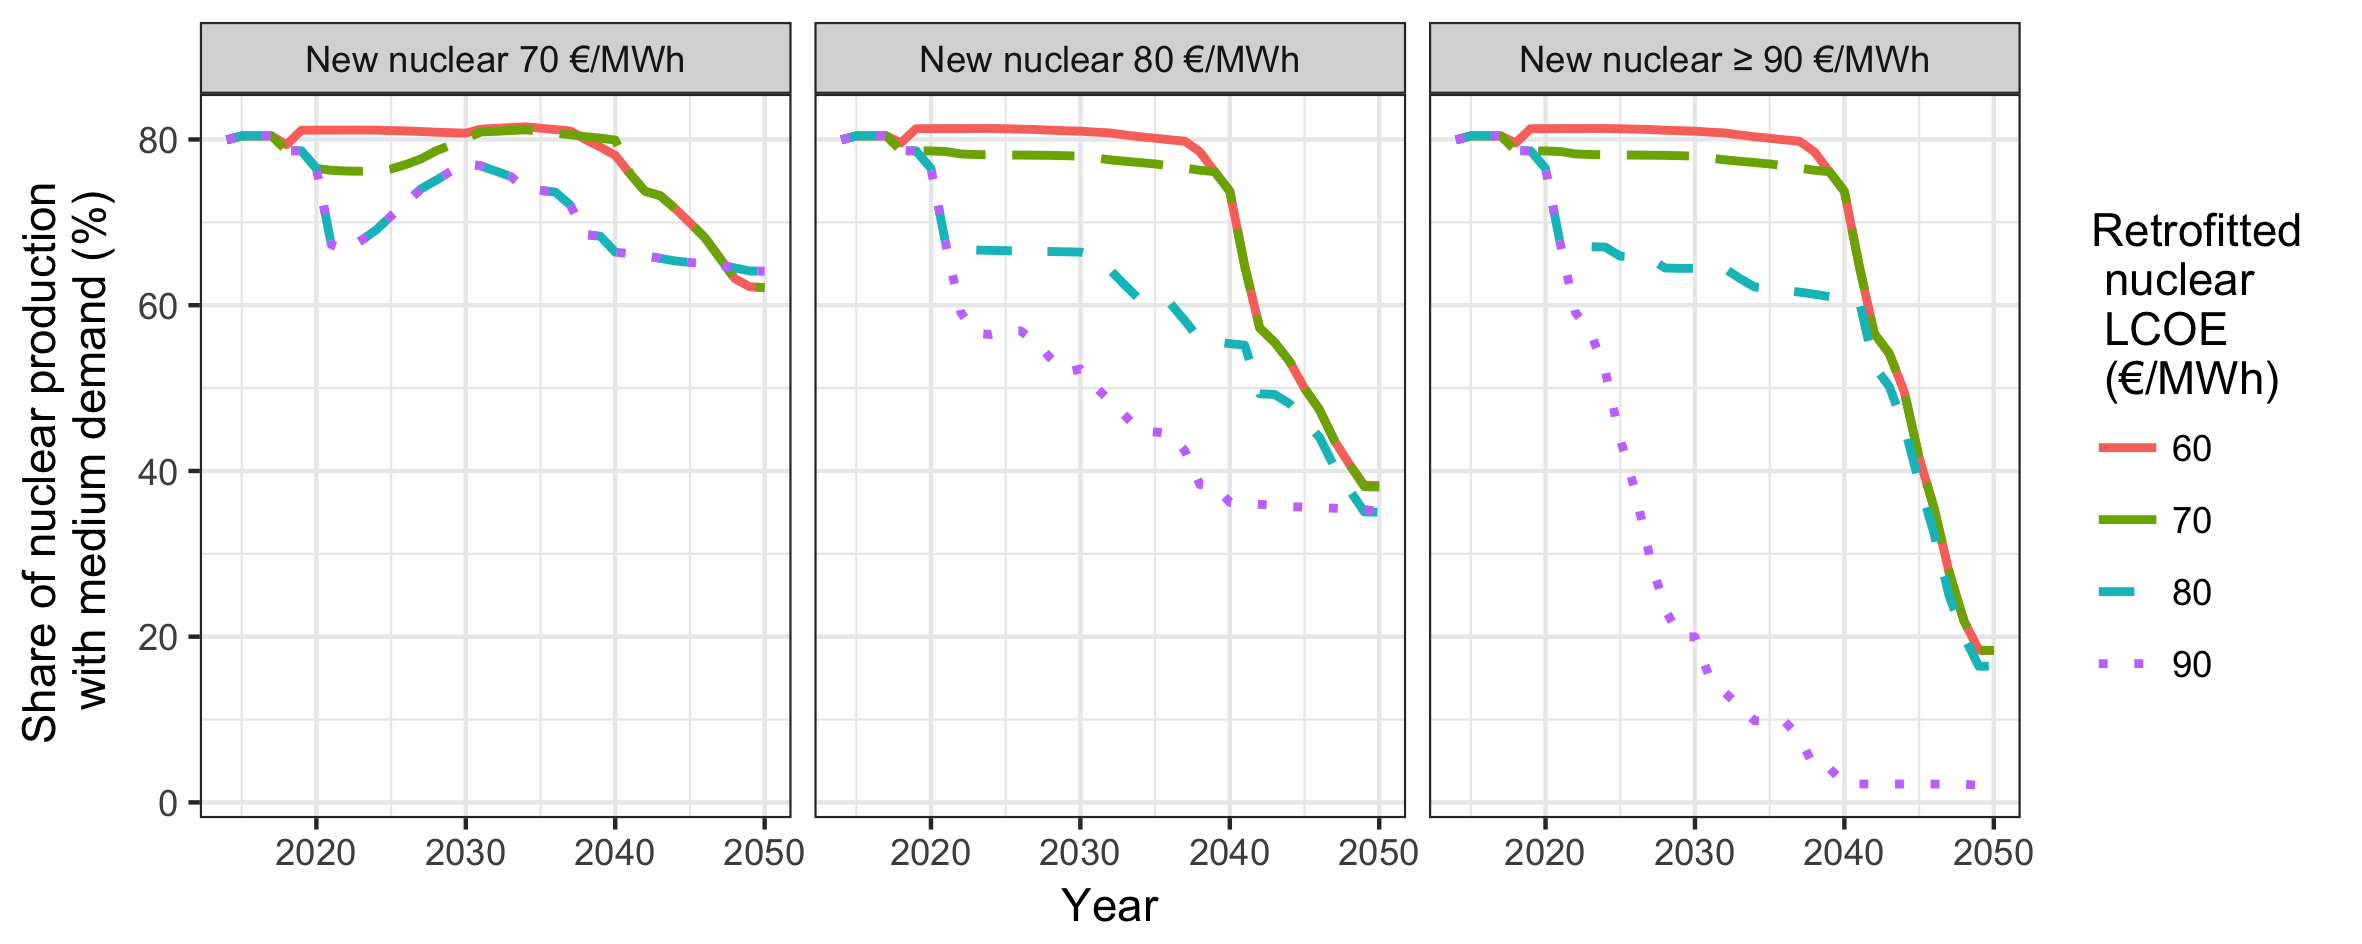
\includegraphics[width=12cm]{figures/nukeShare2_MedD.png}
	\caption{Optimal nuclear share depending on retrofit and new nuclear costs}
	\label{fig:nukeShare}
\end{figure}

From \cref{fig:nukeShare} and the sensitivity analysis on demand in \cref{fig:powerMixSensitivity}, we can conclude that there is not a single optimum in the range of plausible values. On the contrary, the optimal trajectory depends on several uncertain parameters, in particular the production cost of retrofitted nuclear and demand level. Hence, in this case, the framework of cost-minimization and sensitivity analysis does not allow to conclude to a single trajectory. Following our discussion in \cref{sec:method}, this motivates the use of the Robust Decision Making framework developed by \citet{Lempert2006}. We now apply it to find robust strategies, and to highlight the potential trade-offs between various robust strategies.

\subsection{Determine plausible future states}

This first step derives from the litterature review in \cref{sec:plausibleValues}. 
For retrofitted nuclear, we consider that plausible costs range from 40 \emwh\ to 90 \emwh, by step of 10 \emwh. Again, the idea is to encompass a broad initial range in order not to miss any possible value, and the RDM analysis will later identify subsets of costs to draw conclusions. 
As to new nuclear costs, we consider a range from 70 \emwh\ to 110 \emwh, by steps of 20 \emwh. Existing data suggests the cost could be even higher, but since nuclear is not competitive at 110\emwh\ or above in our model, we stop the analysis at this value as it would not add any new information.
For demand, we consider three trajectories drawn from the national debate on energy transition (DNTE): a low, a medium and a high trajectory. They corresponding respectively to the SOB, DIV and DEC scenario, as shown in \cref{fig:DNTE_scenarios}.
Finally, we examine two \coo\ price trajectories: a high trajectory using the official price trajectory from \citet{Quinet2009}, and a low trajectory in which this price is divided by two.
Multiplied by the 27 strategies presented in the next section, these parameter ranges require to run the model 2,916 times. 

These parameters were chosen to study the competitiveness of retrofitted and new nuclear plants. What determines the power mix in our model is the relative competitiveness of nuclear compared to gas and renewables. What matters is not their absolute costs, but their relative costs.
Studying a wide range of costs for nuclear is equivalent to studying a wide cost ratio for nuclear and renewables.
Thus, we choose not to include an additional uncertain input for renewable costs. By doing so, we acknowledge that all results in terms of nuclear costs must be linked to our cost assumptions about renewable power sources, and interpreted in terms of cost ratios.


\subsection{Define a set of strategies}

The second step is to define trajectories of nuclear retrofit. The 58 reactors offer 2\textsuperscript{58}=2.9*$10^{17}$ possibilities. As we aim to test each candidate strategy against multiple values of uncertain parameters, this problem is too computationally intensive. Thus, we simplify it by using a smaller sample of strategies. This sample should represent a variability in the number (or share) of retrofitted reactors, and a variability in the time-dimension as it might be more interesting to retrofit at the beginning (e.g. due higher renewable costs), or at the end (e.g. due to higher \coo\ price).

In order to account for the time-dimension, we split the reactors into three groups, according to the end of their initial 40-year lifetime. The first group includes of all reactors which will reach 40 years before 2021, which means the 14 oldest reactors. The second group includes all reactors reaching 40 years between 2021 and 2025, or 23 reactors. The last group includes the 21 remaining reactors. This split enables to explore whether an early retrofit (or phase-out) should be preferred over a late retrofit (or phase-out). 

To account for the variability in the share of retrofit, we consider three possibilities for each group: i) all reactors are retrofitted; ii) half of the reactors are retrofitted (refurbishing every other reactor from oldest to newest in the group) and iii) no reactor is retrofitted. We end up with 3\textsuperscript{3}=27 different strategies. 
More information on these 27 strategies can be found in appendix \ref{sec:strategies_examined}. Our aim will be to find which of these strategies are robust, performing well in a wide range of futures. 

From a policy point of view, it is important to define now a strategy for the medium-term and even long-term, because investment in retrofitting must be made months or years in advance. It can even be ten years in advance, as the decennial stop related to the mandatory safety check is a good opportunity to start a retrofit. 
This implies that the future of the oldest nuclear plants, starting with Fessenheim, must be decided soon. 
Proposing long-term robust strategies would contribute to the current public debate in France about the decommissioning of this plant, and about the amount of compensations to EDF if the plant were to be closed by a public decision.
In the future, as new information becomes available regarding costs, demand, \coo\ price or any other important parameter, the analysis should be re-runned in an iterative and flexible process.

\subsection{Identify candidate strategies}

The following step is to choose a candidate strategy $s_{candidate}$ that performs well across all futures. Our indicator of performance is the upper-quartile regret. This upper-quartile regret is also the indicator used by \citet{Lempert2006} and \citet{Nahmmacher2016} to pick a candidate strategy. The idea of this indicator is to select a strategy that is not too far from the optimum in 75\% of the cases, i.e. that performs well in most cases -- and we will explore remaining 25\% later by analyzing the vulnerabilities of our candidate strategy. 

Using the costs resulting from our model runs, we compute for each strategy $s \in \mathbb{S}$ its regret in each future state $f \in \mathbb{F}$. Then we compute the upper-quartile regret for each strategy $s$. The results are shown in \cref{fig:regret}. Each dot in the figure shows the regret, in percent, for a strategy $s$ indicated on the x-axis, and a future $f$. The upper-quartile regret is represented by the larger dots. This figure shows that strategy S9 is a good candidate strategy, as it has the lowest upper-quartile regret (3.9\%). S9 is a strategy in which no plant is retrofitted up to 2021 -- which represents an early phase-out for 14 reactors -- but then all other plants are retrofitted.

But \cref{fig:regret} also shows that the strategies S18 and S24 are not far from S9 in terms of regret. Their upper-quartile regret is 4.5\% and 4.2\% respectively. 
S24 is a strategy in which all reactors are retrofitted in the first and third period, but only half of them in the second period. S18 is a strategy in which half the reactors are retrofitted in the first period, and then all of them are retrofitted.
In his paper, \citet{Lempert2006} go on with the RDM analysis considering just one candidate strategy, stating that the final results are not sensitive to the choice of the initial candidate strategy. However, given how close S9, S18 and S24 are in terms of upper-quartile regret, we will perform the rest of the analysis using these three strategies as candidates, in order to make sure our results are not sensitive to the choice of the candidate strategy (S9 is our main candidate strategy, for which will display the figures in the paper, but similar figures for S18 and S24 will be available in the appendix).

\begin{figure}[!ht]
	\centering
	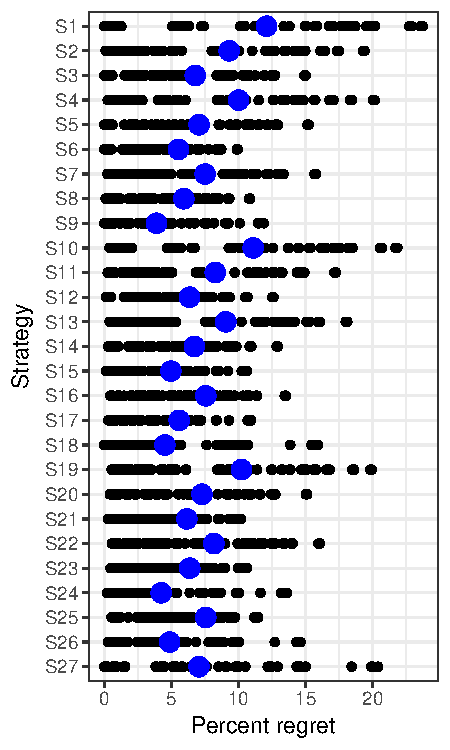
\includegraphics[height=7cm]{figures/regret.pdf}
	\caption{Regret of 27 strategies over 108 plausible states of future}
	\label{fig:regret}
\end{figure}

\subsection{Identify vulnerabilities}

To identify the vulnerabilities of the candidate strategies, we use the Patient Rule Induction Method (PRIM), originally developed by \citet{Friedman1999}. This PRIM algorithm helps identify subsets of parameters in which our target indicator (regret) is above a defined threshold. Documentation on PRIM's operation can be found in \citet{Bryant2010}. We use a public version of the PRIM algorithm implemented in Python in the package called "prim" \citep{Hadka}. 

A regret threshold must be defined to use this PRIM analysis. The ordered distribution of regret shows that regret increases strongly above the threshold 5\% for each candidate strategy S9, S18 and S24 (cf. \cref{fig:quantile_regret}). This value of 5\% corresponds to the 80th centile for S18 and S24, and to the 83th centile for S9, which is close to the upper-quartile regret threshold used by \citet{Nahmmacher2016}. Thus, we choose this value of 5\% as a threshold. 

The PRIM algorithm that, for strategy S9, the most common pattern associated with a regret above 5\% is when retrofit costs is equal to or greater than 80 \emwh in conjunction with a low demand level. These two conditions provide a cluster of states of future $\mathbb{F}_{vuln}(S9)$ to which S9 is vulnerable. Since the states of future in the PRIM-generated clusters do not play in favour of nuclear competitiveness, so we call them "retrofit adverse" states. By opposition, we will call "retrofit friendly" states the remaining states in $\mathbb{F}_{rob}(S9) = \mathbb{F} - \mathbb{F}_{vuln}(S9)$.  

Applying PRIM to strategies S24 and S18 shows that the most common pattern associated with a regret above 5\% is the same for these two strategies: when retrofit costs is equal to or greater than 80 \emwh\ in conjunction with a low \coo\ price and a low to medium demand level. This provides another cluster of "retrofit adverse" states.


\subsection{Characterize trade-offs among strategies}

Identifying vulnerabilities enables us to characterize trade-offs between different strategies. \Cref{fig:low_regret_frontier_S9} compares the upper-quartile regret values for each of the 27 strategies over the two subsets of future states yielded by the PRIM analysis of S9: $\mathbb{F}_{vuln}(S9)$ and $\mathbb{F}_{rob}(S9)$. (The figure with the clusters from S18 and S24 is similar and shown in \cref{fig_app:low_regret_frontier} in appendix).
By switching from one strategy to another, it is possible to lower the regret in one cluster of states, but at the expense of increasing the regret in the other cluster of states. For example, switching from S1 to S10 reduces the regret in "retrofit friendly" states, but increases the regret in "retrofit adverse" states. 
A decision maker can use this figure to choose a strategy that offers the trade-off he prefers. 

From S1 in the upper-left corner to S18 in the bottom-right corner, there is a continuum of available strategies. 
However, some strategies offer a better trade-off than others. 
These strategies are labelled in black. From left to right in the figure, these are S1, S12, S6, S9 and S18. 
They are all located on what can be called a low-regret frontier. 
Some other interesting strategies (though not on the low-regret frontier) are shown in light grey. 
S27 is important as it is the strategy of full retrofit, a policy option often prompted in the public debate. 
It appears that this strategy is far from the low-regret frontier. 
This is due to its vulnerability to a low demand (see \cref{fig_app:vulnerabilities_S27} in the appendix). In other words, retrofitting all existing nuclear plants might lead to a costly overcapacity.

Evidencing this low-regret frontier is an important result, because it enables to select only five strategies as potential robust candidates out of the 27 initial strategies examined. This narrowed choice provides a simpler picture of our initial problem, showing only the strategies with interesting trade-offs.

\begin{figure}[!ht]
	\centering
	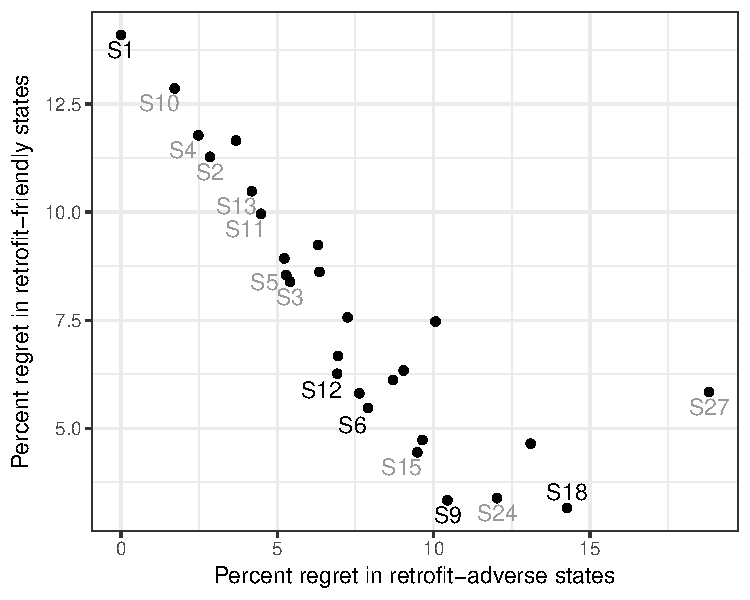
\includegraphics[width=8cm]{figures/low_regret_frontier_S9.pdf}
	\caption{Regret for each strategy in each subset identified}
	\label{fig:low_regret_frontier_S9}
\end{figure}

Having identified the strategies located on the low-regret frontier, the choice of a decision-maker will ultimately depend on his implicit probabilities that a retrofit friendly state occurs. 
This is particularly true for nuclear, which is a controversial source of power, and for which a vast array of costs is plausible. 
If the decision-maker thinks the retrofit friendly cluster is not likely, he will choose to go for S1, the full phase-out strategy; if, on the contrary, he believes the odds of a retrofit friendly state are high, he will pick S18. 

We can simplify the low-regret frontier representation to highlight the most interesting trade-offs between strategy. To that end, we compute the expected regret of a strategy, depending on the relative odds of the two clusters. This is done in \cref{fig:odds_S9} for the clusters from strategy S9. This figure shows that there are four main options which can claim to be optimal, depending on the implicit probabilities of the decision maker. 
The x-axis shows the odds of the "retrofit adverse" states versus the odds of the "retrofit friendly" states. 
The y-axis shows the regret associated with each strategy and implicit odds. 
The target of a decision-maker is to pick a strategy with the lowest regret. 
If he believes that a retrofit friendly state is unlikely (odds below 1:1), he should pick strategy S1. 
On the contrary, if he believes that a retrofit friendly" state is certain, he should pick strategy S18.
If he believes that a retrofit friendly state is more likely but not certain, he should pick strategy S9.
Finally, there is a case in which strategy S12 would be picked: if the decision maker thinks the odds are very close to 1:1.
If we use the PRIM-generated clusters based on strategy S18 and S24, the results are similar, except that strategy S12 is replaced with strategy S6. This is shown in \cref{fig_app:odds} in the appendix.


\begin{figure}[!ht]
	\centering
	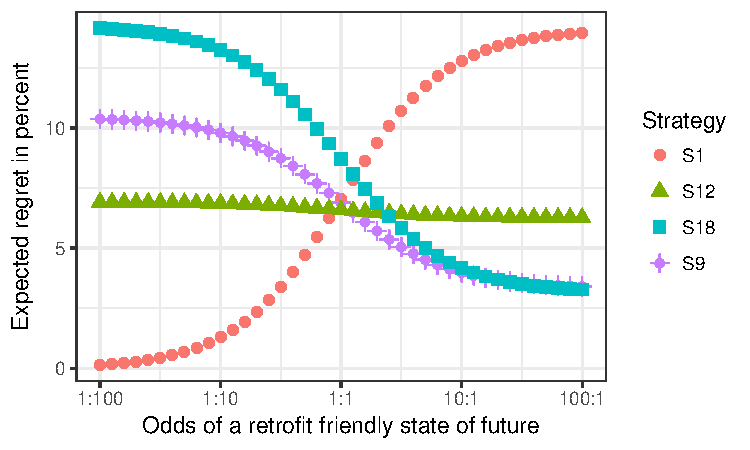
\includegraphics[width=8cm]{figures/odds_S9.pdf}
	\caption{Expected regret of low-regret strategies depending on the implicit probabilities of a decision maker}
	\label{fig:odds_S9}
\end{figure}

The results shown in \cref{fig:odds_S9} do not try to settle the debate on nuclear. On the contrary, they show that various strategies can be considered as optimal from a cost-minimization perspective. This helps understand the coexistence of various opinions. But they also provide a quantified framework which accounts for uncertainty to support policy decision. 

Currently, the cost of retrofitted nuclear is estimated at around 40 \emwh\ by EDF. Although there is a lot of uncertainty about that figure, a cost of retrofitted nuclear below 80 \emwh\ seems more likely today. Thus, strategies S9 and S18 seem to be the best robust strategies given current cost estimates, in the sense that they yield the lowest expected regret over a large range of the most plausible future states.

S9 and S18 are close strategies: they are both based on a full retrofit after 2021. The difference is that S18 include to retrofit 50\% of the 14 oldest plants, while S9 plans to retrofit none. 
Both strategies yield the lowest regret in the most likely future states, as shown in \ref{fig:low_regret_frontier_S9}, providing a good hedge against higher than expected cost of nuclear, low demand of low carbon price. 
Choosing between S9 and S18 will be a matter of implicit probability of the decision maker. S18 is slightly more performing if nuclear is below 60 \emwh and demand is flat or increasing. But S9 performs better if demand is low, and it is less vulnerable to an increase in retrofit costs in conjunction with a low \coo\ price (cf. \cref{fig_app:vulnerabilities_S9_S18_S27} in appendix).

In conclusion, we have evidenced that the most robust strategies imply an early-phase out of 7 to 14 out of the 14 oldest reactors, given the current estimates of cost, demand and \coo\ price. The intuition behind these results comes from a balance between risks and costs. On one hand, retrofitting all plants is a strategy vulnerable to lower demand or higher than expected costs of retrofit. On the other hand, nuclear provides a low-carbon, flexible source of electricity. Higher share of renewables entails a drop in the value of their production, due to autocorrelation and increasing flexibility burden for the system. This reduces their competitiveness as their penetration rate increases. Our analysis has revealed two robust strategies in-between these two extremes, which imply closing 7 to 14 reactors. 
We also highlighted their vulnerabilities, their alternatives, and the potential trade-offs with other strategies. Our approach keeps the debate open, as we highlight that other strategies might be considered cost-optimal for assumptions less in line with the literature, but still plausible given the current uncertainty. 
The final choice of a strategy will ultimately depend on the implicit probabilities perceived by the decision-maker. We thus contribute to the debate on nuclear in France, in particular with respect to the retrofit of the nuclear plants of Fessenheim and Bugey, which will reach 40 years in 2017 and 2018 respectively.


%%%%%%%%%%%%%%%%%%

\section{Comparison with French official scenarios}
\label{sec:comparison}

\subsection{Presentation of the official scenarios}

From 2012 to 2015, France engaged in a National Debate on the Energy Transition (\dnte), which finally led to a new "Law on the Energy Transition for a Green Growth"\footnote{
	Loi 2015-992 du 17 août 2015 relative à la transition énergétique pour la croissance verte.
}.
A discussion on the future of the energy mix brought together various political stakeholders, as well as unions and NGOs.
During the debate, the power mix and the share of nuclear were a point of particular focus, with a dedicated working group. Eleven energy transition scenarios were created by the different parties to promote their own vision of France's energy landscape, and these scenarios were ultimately grouped into four representative scenarios.

These four scenarios represent the different views that existed in 2012, and they have been structuring the French debate on nuclear ever since. The rationale of each representative scenario is summarized in \cref{tab:dnteScenarios}, but more information can be found in \citet{DNTE_gt2}.
Quantitatively, each scenario can be defined by two criteria: demand level and nuclear share, as detailed in \cref{fig:DNTE_scenarios}.

\begin{table}
	%\colorTable
	\begin{tabular}{p{2cm}p{6cm}cp{2.5cm}}
		\toprule
		Scenario name & Scenario description & Demand & Nuclear Share \\
		\midrule
		Sobriety (SOB)     	& A strong energy efficiency and sobriety reduce power demand.\newline Nuclear and fossil fuels are phased out. & Strong decrease & Full phase-out \\
		Efficiency (EFF)  	 & Ambitious energy efficiency targets and diversification of power sources & Slight decrease & Decrease to 50\% in 2030 and 25\% in 2040 \\
		Diversification (DIV) 	& Diversification of power sources & Slight increase & Decrease to 50\% from 2030 onwards \\
		Decarbonation (DEC)  & High power demand due to increase electrification and high nuclear share & Strong increase & Full retrofit \\
		\bottomrule
	\end{tabular}
	\caption{\label{tab:dnteScenarios}DNTE scenarios}
\end{table}


\subsection{Robust vs official scenarios}
Based on these criteria of demand level and nuclear share, we can find which strategy among the 27 studied in this paper would best represent each official scenario. 
The DEC scenario corresponds to a retrofit of all nuclear plants. The SOB scenario is a scenario of full phase-out. Thus, their equivalent strategies are S27 and S1 respectively. But a methodology is required to determine the equivalent strategy of the EFF and DIV scenarios. 
To that end, we combine the information on nuclear share and demand level in each scenario to deduct the annual nuclear power generation in 2020, 2030 and 2040.
Generation is used as a proxy to estimate the number of retrofitted plants (it is a better proxy than nuclear share, as it accounts for the differences in demand level between the four scenarios of the DNTE). Based on the three years 2020, 2030 and 2040, we compute the distance between the nuclear production in each strategy and the nuclear production in the DNTE scenarios. Distance $D$ is defined here as the square root of the sum of squared difference in nuclear production for each year:
$$D(\text{strategy, DNTE scenario}) = \sqrt{ \sum_{\text{y in {2020,2030,2040}}} (Prod^y_{\text{strategy}} - Prod^y_{\text{scenario DNTE}})^2}$$
where $Prod^y$ is the production in year $y$.
With this methodology, the best matches for the EFF and DIV scenarios are S13 and S6 respectively. In addition, this distance-based methodology gives respectively S1 and S27 as best estimates for the SOB and DEC scenarios, as expected.

Now that we have identified which strategy matches each scenario of the DNTE, we can build on our previous analysis. \Cref{fig:low_regret_frontier_S9} shows that the four DNTE scenarios (S1, S13, S6, S27) cover well the spectrum of possible trade-offs: S1 and S27 are the two extreme points of full phase-out and full retrofit respectively. S13 and S6 provide more balanced intermediate points, with a retrofit share of 27\% and 63\% respectively. Thus, the DNTE scenarios offers a representative panel of the policy options available in terms of capacity decommissioned.

However, our RDM analysis has also revealed the shortcomings of the DNTE scenarios and the contribution of our RDM analysis. 
First, we showed that the full-retrofit option, DEC (S27), is not a low-regret option. This is due to its high vulnerability to a decreasing demand. This is an important result because the full retrofit is often presented as the cheapest policy option in the public debate.
Second, we explored 27 strategies instead of just four scenarios, and we highlighted their trade-offs given implicit assumptions about the future cost of nuclear. 
Results from a pure cost-minimization framework can only state what is the optimal power mix given a fixed set of assumptions on costs, demand, \coo\ price, etc. But since there is uncertainty on these parameters, the message is not easily transformed into a policy advise.

With RDM analysis, we simplified a multidimensional problem to a simple trade-off between two possible clusters of future states. We show the trade-offs in terms of implicit probabilities, providing a message more readable and easier to use by decision makers: "if you think a retrofit friendly state is likely, you should aim for S9; if you think it is certain, pick S18; if you think it is unlikely, pick S1". 
Finally, we showed that two strategies in particular, S9 and S18, are likely to provide the lowest regret --given current cost estimates-- over a large range of the most plausible future states. These robust strategies consist in decommissioning 7 to 14 of the 14 oldest reactors, and then retrofit all the remaining ones. These are two intermediate paths that were missing in the four official scenarios. Currently, the options were either to retrofit all plants or close more than 30 reactors. Thus, we have evidenced two new robust strategies. This could contribute to the public debate in France, and in other countries where the decision to retrofit or decommission nuclear power plants is discussed.

%%%%%%%%%%%%%%%%%%



\section{Conclusion}
\label{sec:conclusion2}

After the first oil shock, France launched the world’s largest nuclear program, ordering 36 reactors within two years, and 58 reactors in total. These reactors are now reaching the end of their technological lifetime. But extending these lifetimes requires an investment up to \euro 100 billion by 2030. 
France is thus at a crossroads and must define a new nuclear policy. The economics of this decision crucially depend on several parameters, in particular the future costs of nuclear (including decommissioning, waste and insurance), demand levels and the social cost of carbon, all of which are subject to significant uncertainty.

In face of all these uncertainties, we apply the framework of Robust Decision Making (RDM) to find a robust strategy indicating which plants should be retrofitted.

Based on nearly 3,000 runs, our analysis revealed two robust strategies, which imply the early-phase out of between 7 and 14 of the 14 oldest reactors. We also assessed the vulnerabilities and alternatives of such a strategy, as well as the potential trade-offs with other strategies. Our approach keeps the debate open: we highlight that several options exist depending on the implicit probabilities of decision-makers. But considering the current estimates of cost, demand and carbon price, the two aforementioned strategies are likely to yield the lowest regret. 

Our policy recommendation differs from the official French government scenarios which stem from the national debate. Our analysis has thus revealed new, robust strategies. It provides a timely contribution to the debate on nuclear in France, in particular with respect to the retrofit of the nuclear plants of Fessenheim, which will reach 40 years in 2017.

Our framework could be used iteratively in the future. Each time the decision to retrofit a nuclear plant has to be made, the same analysis could be run. The advantage would be to benefit from newer information on costs, the level of electricity demand or the social cost of carbon.

